\notechapter{N-20261124}{Tensors, Degenerations, and the Nine-Fourths Exponent}

Multiplying two \(n \times n\) matrices looks at first glance like a rigid, elementary calculation requiring \(n^3\) scalar multiplications. Yet the moment we rewrite matrix multiplication as a trilinear tensor, the problem leaves concrete algorithms behind and turns into a question about algebraic geometry, semiring homomorphisms, and asymptotic degenerations.

\begin{question}[title={The structural puzzle behind \(\omega = 9/4\)}]
The matrix multiplication exponent \(\omega\) is governed by the asymptotic rank of a single family of tensors \(\langle n, n, n \rangle\). Why does a seemingly innocuous rational number, \(\frac{9}{4} = 2.25\), emerge as the exact threshold? What algebraic trick forces \(\omega \le 9/4\) from above, and what geometric obstruction blocks any algorithm from crossing \(9/4\) from below?
\end{question}

The October 2026 upper bound was followed by a manuscript dated November 24, 2026 claiming a matching lower bound over every field in the formal arithmetic-circuit model, with a Lean formalization of the division-free square exponent.\footnote{OpenAI, \emph{An Upper Bound of \(9/4\) for the Matrix Multiplication Exponent}, October 2, 2026, \href{https://github.com/openai/math/tree/main/preprints/Matrix-Multiplication-Nine-Fourths-October-2-2026}{manuscript}; OpenAI, \emph{The matrix multiplication exponent is nine fourths}, November 24, 2026, \href{https://github.com/openai/math/tree/main/preprints/The-matrix-multiplication-exponent-is-nine-fourths-November-24-2026}{manuscript and proof artifacts}. This note does not independently verify the full lower-bound geometric machinery.} We focus on the mathematical architecture behind the \(9/4\) threshold. Rather than tracing chronological records, we build the tensor-semiring machinery from scratch, inspect how \vocab{border rank} and \vocab{Strassen's asymptotic spectrum} convert complexity into real-valued homomorphisms, isolate the algebraic mechanism of \vocab{separating a shared tensor leg}, and contrast the upper-bound squeeze with the dual picture of \vocab{tensor-network incompressibility}.

\section{The algebraic stage: tensors, rank, and border rank}

\subsection{Matrix multiplication and polynomial multiplication as tensors}

Fix a base field \(\FF\). A bilinear map \(\beta : U^* \times V^* \to W\) between finite-dimensional \(\FF\)-vector spaces corresponds canonically to a \(3\)-tensor
\[
  T \in U \otimes V \otimes W.
\]
Two families of tensors serve as the protagonists of this note.

\begin{definition}[Matrix multiplication and polynomial multiplication tensors]
\label{def:mm-nine-fourths-two-tensors}
\begin{enumerate}
  \item For positive integers \(n, m, p\), the \vocab{matrix multiplication tensor} \(\langle n, m, p \rangle \in \FF^{n\times m} \otimes \FF^{m\times p} \otimes \FF^{p\times n}\) is defined in standard matrix-unit bases by
  \[
    \langle n, m, p \rangle \defeq \sum_{i=1}^{n} \sum_{j=1}^{m} \sum_{k=1}^{p} e_{i,j} \otimes e_{j,k} \otimes e_{k,i}.
  \]
  Viewing \(\langle n, m, p \rangle\) as a trilinear form on \(\Mat_{n\times m}(\FF) \times \Mat_{m\times p}(\FF) \times \Mat_{p\times n}(\FF)\), it is simply the cyclic trace
  \[
    (A, B, C) \longmapsto \Tr(ABC) = \sum_{i,j,k} A_{ij} B_{jk} C_{ki}.
  \]
  \item For positive integers \(a, b\), the \vocab{polynomial multiplication tensor} (discrete linear convolution) \(P_{a,b} \in \FF^a \otimes \FF^b \otimes \FF^{a+b-1}\) is
  \[
    P_{a,b} \defeq \sum_{i=0}^{a-1} \sum_{j=0}^{b-1} e_i \otimes e_j \otimes e_{i+j},
  \]
  encoding the product of a polynomial of degree \(< a\) with one of degree \(< b\).
  \item For \(r \in \NN\), the \vocab{unit tensor} of size \(r\) is \(\langle r \rangle \defeq \sum_{i=1}^r e_i \otimes e_i \otimes e_i \in \FF^r \otimes \FF^r \otimes \FF^r\).
\end{enumerate}
\end{definition}

Writing \(\langle n, m, p \rangle\) via \(\Tr(ABC)\) makes an otherwise hidden symmetry immediate: because \(\Tr(ABC) = \Tr(BCA) = \Tr(CAB)\), cyclic permutation of the three tensor factors maps \(\langle n, m, p \rangle\) isomorphically onto \(\langle m, p, n \rangle\) and \(\langle p, n, m \rangle\). Likewise, notice the boundary degeneration of polynomial multiplication: when \(a = 1\), the map \((x_0, (y_0,\dots,y_{b-1})) \mapsto (x_0 y_0, \dots, x_0 y_{b-1})\) is literally \(1\times 1\) by \(1\times b\) matrix multiplication, so
\begin{equation}
  P_{1,b} \cong \langle 1, 1, b \rangle,
  \qquad
  P_{a,1} \cong \langle a, 1, 1 \rangle.
  \label{eq:mm-nine-fourths-P1b}
\end{equation}

\subsection{The tensor semiring, restriction, and degeneration}

Up to mutual restriction (after removing unused ambient directions), \(3\)-tensors over \(\FF\) form a commutative semiring \((\mathcal{T}, \oplus, \otimes)\):
\begin{itemize}
  \item The \vocab{direct sum} \(S \oplus T \in (U_1 \oplus U_2) \otimes (V_1 \oplus V_2) \otimes (W_1 \oplus W_2)\) represents computing \(S\) and \(T\) on completely independent inputs and outputs.
  \item The \vocab{Kronecker (tensor) product} \(S \otimes T \in (U_1 \otimes U_2) \otimes (V_1 \otimes V_2) \otimes (W_1 \otimes W_2)\) satisfies the key block-multiplication identity
  \[
    \langle n_1, m_1, p_1 \rangle \otimes \langle n_2, m_2, p_2 \rangle
    \cong \langle n_1 n_2,\, m_1 m_2,\, p_1 p_2 \rangle.
  \]
\end{itemize}

To compare the computational cost of two tensors, we introduce two preorders on \(\mathcal{T}\).

\begin{definition}[Restriction, degeneration, rank, and border rank]
\label{def:mm-nine-fourths-preorders}
Let \(S \in U_1 \otimes V_1 \otimes W_1\) and \(T \in U_2 \otimes V_2 \otimes W_2\).
\begin{itemize}
  \item We say \(S\) is a \vocab{restriction} of \(T\), written \(S \le T\), if there exist linear maps \(A : U_2 \to U_1\), \(B : V_2 \to V_1\), \(C : W_2 \to W_1\) such that \((A \otimes B \otimes C)(T) = S\).
  \item We say \(S\) is a \vocab{degeneration} of \(T\), written \(S \trianglelefteq T\), if there exist polynomial-entry linear maps \(A(\eps), B(\eps), C(\eps)\) over \(\FF[\eps]\) and an integer \(d \ge 0\) such that
  \[
    \bigl(A(\eps) \otimes B(\eps) \otimes C(\eps)\bigr)(T) = \eps^d S + O(\eps^{d+1})
  \]
  as a polynomial in \(\eps\).
  \item The \vocab{tensor rank} \(R(T)\) is the minimum \(r\) such that \(T \le \langle r \rangle\); equivalently, the smallest number of simple tensors \(u_i \otimes v_i \otimes w_i\) summing to \(T\).
  \item The \vocab{border rank} \(\underline{R}(T)\) is the minimum \(r\) such that \(T \trianglelefteq \langle r \rangle\).
\end{itemize}
\end{definition}

The \vocab{matrix multiplication exponent} over \(\FF\) is then
\begin{equation}
  \omega(\FF) \defeq \inf \bigl\{\, \tau \in \RR : R(\langle n, n, n \rangle) = O(n^\tau) \,\bigr\}
  = \lim_{n \to \infty} \frac{\log R(\langle n, n, n \rangle)}{\log n}.
  \label{eq:mm-nine-fourths-omega-def}
\end{equation}

\begin{caution}[title={Infimum versus minimum}]
By definition, \(\omega(\FF) = 9/4\) asserts that for every \(\delta > 0\) there exists a bilinear algorithm computing \(n \times n\) matrix products in \(O_\delta(n^{9/4 + \delta})\) scalar multiplications, while no algorithm can achieve \(O(n^{9/4 - \delta})\). It does \emph{not} by itself decide whether \(R(\langle n,n,n\rangle) = O(n^{9/4})\) without the extra \(n^\delta\) or polylogarithmic factors.
\end{caution}

\subsection{Why degeneration strictly beats exact rank: the \(W\)-tensor}

At first sight, letting \(\eps \to 0\) in Definition~\ref{def:mm-nine-fourths-preorders} looks like numerical cheating. In fact, it is a pure algebraic operation over \(\FF[\eps]\) that strictly enlarges the set of available reductions, and the extra \(\eps\)-polynomial overhead disappears completely in the asymptotic exponent.

\begin{example}[The \(W\)-tensor has rank \(3\) and border rank \(2\)]
\label{ex:mm-nine-fourths-W-tensor}
Consider the symmetric tensor in \(\FF^2 \otimes \FF^2 \otimes \FF^2\) given by
\[
  W \defeq e_0 \otimes e_0 \otimes e_1 + e_0 \otimes e_1 \otimes e_0 + e_1 \otimes e_0 \otimes e_0.
\]
Expanding the difference of just \emph{two} rank-\(1\) tensors over \(\FF[\eps]\), we obtain
\[
  (e_0 + \eps e_1)^{\otimes 3} - e_0^{\otimes 3}
  = \eps W + \eps^2 (e_0 \otimes e_1 \otimes e_1 + e_1 \otimes e_0 \otimes e_1 + e_1 \otimes e_1 \otimes e_0) + \eps^3 e_1^{\otimes 3}.
\]
Thus \(W \trianglelefteq \langle 2 \rangle\), proving \(\underline{R}(W) = 2\). On the other hand, one checks directly by slicing along the first leg that \(R(W) = 3\): the two slices \(M_0 = e_0 \otimes e_1 + e_1 \otimes e_0\) and \(M_1 = e_0 \otimes e_0\) span a \(2\)-dimensional space of \(2 \times 2\) matrices containing no rank-\(1\) matrix other than multiples of \(M_1\), so \(M_0\) and \(M_1\) cannot both lie in the span of two rank-\(1\) matrices.
\end{example}

Notice the mechanism in Example~\ref{ex:mm-nine-fourths-W-tensor}: unwanted cross-terms are not forced to vanish identically; they are merely pushed into higher powers of \(\eps\), where they vanish modulo \(\eps^{d+1}\). Exactly this weighted-vanishing trick powers the separation of shared tensor legs in Section~3.

\section{Strassen's asymptotic spectrum}

Direct computation of \(R(T)\) or \(\underline{R}(T)\) is notoriously wild: rank is neither multiplicative under \(\otimes\) nor additive under \(\oplus\) in general. Volker Strassen's key insight was to pass to the \emph{asymptotic} preorder: write \(S \lesssim T\) if \(S^{\otimes N} \le T^{\otimes (N + o(N))}\) as \(N \to \infty\). On the resulting ordered semiring, asymptotic complexity is completely governed by real-valued semiring homomorphisms.

\begin{definition}[Asymptotic spectrum of tensors]
\label{def:mm-nine-fourths-spectrum}
The \vocab{asymptotic spectrum} \(\Delta(\mathcal{T})\) is the set of all maps \(\phi : \mathcal{T} \to \RR_{\ge 0}\) satisfying, for all \(S, T \in \mathcal{T}\):
\begin{enumerate}
  \item \(\phi(S \oplus T) = \phi(S) + \phi(T)\),
  \item \(\phi(S \otimes T) = \phi(S)\,\phi(T)\),
  \item \(S \le T \implies \phi(S) \le \phi(T)\),
  \item \(\phi(\langle 1 \rangle) = 1\).
\end{enumerate}
Elements \(\phi \in \Delta(\mathcal{T})\) are called \vocab{spectral points} (or \vocab{tensor characters}).
\end{definition}

Over an infinite field, every spectral point is monotone under degeneration. If the polynomial family realizing \(S\trianglelefteq T\) has degree at most \(L\), its \(N\)-th tensor power has first nonzero coefficient \(S^{\otimes N}\) and degree at most \(NL\). Interpolation extracts this coefficient as a linear combination of at most \(NL+1\) restrictions of \(T^{\otimes N}\). Hence \(\phi(S)^N\leq(NL+1)\phi(T)^N\); taking \(N\)-th roots proves \(\phi(S)\leq\phi(T)\). The upper-bound argument may therefore take place over the algebraic closure.

\begin{theorem}[Strassen's asymptotic spectrum duality]
\label{thm:mm-nine-fourths-strassen-duality}
For every tensor \(T \in \mathcal{T}\), its asymptotic rank \(\tilde{R}(T) \defeq \lim_{N\to\infty} R(T^{\otimes N})^{1/N}\) satisfies
\[
  \tilde{R}(T) = \max_{\phi \in \Delta(\mathcal{T})} \phi(T).
\]
In particular, the matrix multiplication exponent is given by
\[
  \omega(\FF) = \sup_{\phi \in \Delta(\mathcal{T})} \log_2 \phi(\langle 2, 2, 2 \rangle).
\]
\end{theorem}

\subsection{Directional exponents and six-fold symmetrization}

Write \(B_X(m)=\langle1,1,m\rangle\), \(B_Y(m)=\langle m,1,1\rangle\), and \(B_Z(m)=\langle1,m,1\rangle\). The subscript denotes the one-dimensional leg, while the other two carry a dot product of dimension \(m\). For each such family, the character is completely multiplicative in \(m\), nondecreasing, and bounded between \(1\) and \(m\). Comparing powers of any two integers thus gives
\[
 \phi(B_X(m))=m^{p_X},\quad
 \phi(B_Y(m))=m^{p_Y},\quad
 \phi(B_Z(m))=m^{p_Z},
\]
where the three exponents lie in \([0,1]\). The product identity for matrix multiplication yields
\[
 \phi(\langle n,m,p\rangle)=n^{p_Y}m^{p_Z}p^{p_X}.
\]
Set \(t=(p_X+p_Y+p_Z)/3\). Then
\begin{equation}
 \phi(\langle n,n,n\rangle)=n^{3t}.
 \label{eq:mm-nine-fourths-theta}
\end{equation}
A unit tensor of size \(n\) restricts from \(\langle n,n,n\rangle\), so \(t\geq1/3\).

There is no reason for an arbitrary spectral point to assign equal values to the three dot products. For \(\pi\in S_3\), put \(\phi_\pi(T)=\phi(T^\pi)\), the character obtained by permuting the legs. Each directional exponent occurs twice among the six first-leg exponents, and therefore
\[
 \sum_{\pi\in S_3}p_X^{(\pi)}=6t.
\]
We will apply inequalities to these six characters individually before combining their values. Their geometric mean is not assumed additive.

\subsection{Polynomial interpolation and the normalized profile}

\begin{lemma}[Vandermonde restriction]
\label{lem:mm-nine-fourths-vandermonde}
If the field contains at least \(a+b-1\) distinct elements, then \(R(P_{a,b})=a+b-1\).
\end{lemma}
\begin{proof}
Evaluate both polynomials at \(a+b-1\) distinct points, multiply corresponding evaluations, and interpolate the product coefficients. This gives the upper bound. The output flattening has rank \(a+b-1\), since all output degrees occur and their slices have disjoint supports.
\end{proof}

For a fixed character, introduce the symmetrized convolution profile
\begin{equation}
 P(a,b)=\left(\prod_{\pi\in S_3}\phi_\pi(P_{a,b})\right)^{1/(6t)}.
 \label{eq:mm-nine-fourths-Pab-norm}
\end{equation}
Interchanging input legs permutes the six factors. Since \(P_{1,b}=B_X(b)\) up to isomorphism, and interpolation bounds each character by \(a+b-1\), we have
\begin{equation}
 P(a,b)=P(b,a),\quad P(1,b)=b,\quad
 P(a,b)\leq(a+b-1)^{1/t}.
 \label{eq:mm-nine-fourths-upper-anchor}
\end{equation}

\section{Separating a shared tensor leg}

To force the \(9/4\) exponent, we need two inequalities:
\begin{align}
 2P(a,b)&\geq P(a,b-1)+P(a,b+1) &&(b\geq2),\label{eq:mm-nine-fourths-concavity}\\
 P(a,3h+a-1)&\geq3P(a,h).\label{eq:mm-nine-fourths-recurrence}
\end{align}
Both originate from the same idea: separate blocks whose second and third legs are already independent, while retaining an auxiliary dot product. The following proofs develop the October 2026 manuscript's Sections 3--5.

\subsection{The shared-leg obstruction and Fourier separation}

Consider \(T=\sum_{h=1}^M T_h\), where \(T_h\in X\otimes Y_h\otimes Z_h\), the \(Y_h\) and \(Z_h\) are disjoint sectors, and \(X\) is common. Additivity of a character does not apply to this sum. One can separate the shared leg by a naive restriction using an auxiliary dot product, but that consumes a factor growing with \(M\). Instead, we use \(O(M)\) copies of the source and preserve a dot product of size \(M\) in each separated block.

\begin{proposition}[Finite shared-leg separation]
\label{prop:mm-nine-fourths-separate}
For the matched-sector tensor above,
\[
 \bigoplus_{h=1}^M(T_h\otimes B_X(M))
       \trianglelefteq T^{\oplus L},\qquad L=5M
\]
over \(\CC\). Over an algebraically closed field of positive characteristic, choose \(L\in\{5M,5M+1\}\) coprime to the characteristic.
\end{proposition}
\begin{proof}
Write the trilinear form as \(\sum c_{hijk}x_i y_{h,j}z_{h,k}\), and choose a primitive \(L\)-th root of unity \(\zeta\). In copy \(r\), with \(0\leq r<L\), substitute
\begin{align*}
 x_i^{(r)}&\mapsto\sum_{g=1}^M\zeta^{2rg}X_{i,g},\\
 y_{h,j}^{(r)}&\mapsto\sum_{u=1}^M\zeta^{r(u-h)}Y_{h,j,u},\\
 z_{h,k}^{(r)}&\mapsto L^{-1}\sum_{v=1}^M\zeta^{-r(v+h)}Z_{h,k,v}.
\end{align*}
The sum over \(r\) retains exactly the indices satisfying
\[
 u-v+2(g-h)=0,
\]
because their Fourier phase vanishes modulo \(L\) and the expression has absolute value at most \(3(M-1)<L\).

Give \(X_{i,g},Y_{h,j,u},Z_{h,k,v}\) the respective \(\eps\)-weights
\[
 g^2,\qquad hu-h^2,\qquad -hv.
\]
On every term surviving the Fourier projection, the sum of the weights is
\[
 g^2-h^2+h(u-v)=(g-h)^2.
\]
Thus the zero-weight coefficient has \(g=h\), and then \(u=v\). It is
\[
 \sum_{h,i,j,k,u}c_{hijk}X_{i,h}Y_{h,j,u}Z_{h,k,u}.
\]
Every leg now distinguishes the sector label \(h\); the repeated index \(u\) gives the extra dot product. Negative individual weights are harmless: a common shift on each leg turns all substitutions into polynomial maps, merely shifting the leading degree.
\end{proof}

\begin{figure}[htbp]
\centering
\begin{tikzpicture}[>=Stealth,font=\small]
 \fill[MidnightBlue!15] (0,0) rectangle (2.7,.4);
 \draw[MidnightBlue,thick] (0,0) rectangle (2.7,.4);
 \node[below] at (1.35,0) {shared \(X\)};
 \foreach \i/\c in {0/purple,1/teal,2/RawSienna}{
   \draw[dashed,gray] (.45+.9*\i,.4)--(.45+.9*\i,1.2);
   \fill[\c!20] (.1+.9*\i,1.2) rectangle (.8+.9*\i,1.8);
   \draw[\c!80!black,thick] (.1+.9*\i,1.2) rectangle (.8+.9*\i,1.8);
 }
 \node[above] at (1.35,1.8) {\(L\) source copies};
 \draw[->,very thick,MidnightBlue] (3,1.05)--(5.1,1.05);
 \node[above,align=center] at (4.05,1.1) {Fourier filter\\ \(\eps^{(g-h)^2}\)};
 \foreach \i/\c in {0/purple,1/teal,2/RawSienna}{
   \fill[\c!20] (5.5+.9*\i,1.2) rectangle (6.2+.9*\i,1.8);
   \draw[\c!80!black,thick] (5.5+.9*\i,1.2) rectangle (6.2+.9*\i,1.8);
   \fill[MidnightBlue!15] (5.5+.9*\i,.62) rectangle (6.2+.9*\i,.92);
   \draw[MidnightBlue,thick] (5.5+.9*\i,.62) rectangle (6.2+.9*\i,.92);
   \draw[gray] (5.85+.9*\i,.92)--(5.85+.9*\i,1.2);
 }
 \node[above] at (6.75,1.8) {private blocks};
 \node[below] at (6.75,.55) {\(T_h\otimes B_X(M)\)};
\end{tikzpicture}
\caption{Separation retains a dot product in each independent output block. The Fourier filter constrains the labels and the quadratic weight eliminates precisely their mismatches.}
\label{fig:mm-nine-fourths-shared-leg}
\end{figure}

\begin{lemma}[Entropy gain from partially direct sums]
\label{lem:mm-nine-fourths-entropy}
For nonzero matched sectors \(T_1,\ldots,T_s\) sharing their first leg and any probability vector \(q\),
\[
 \phi(T)\geq e^{p_X H(q)}\prod_{i=1}^s\phi(T_i)^{q_i},
 \qquad H(q)=-\sum_i q_i\log q_i.
\]
\end{lemma}
\begin{proof}
First take rational \(q\) and powers \(N\) with \(Nq_i\) integral. Restrict \(T^{\otimes N}\) to sector words having exactly \(Nq_i\) occurrences of label \(i\). There are \(M_N=N!/\prod_i(Nq_i)!\) matched sectors, each with character \(C_N=\prod_i\phi(T_i)^{Nq_i}\). Finite separation and monotonicity give
\[
 L\,\phi(T)^N\geq M_N^{1+p_X}C_N,\qquad L=O(M_N).
\]
Divide by \(M_N\), take \(N\)-th roots and use Stirling's formula, \(\log M_N/N\to H(q)\). Rational approximation gives the result for all probability vectors.
\end{proof}

\subsection{The determinant filtration: discrete concavity}

Let \(V_e=\FF[u,v]_e\) be the space of degree-\(e\) homogeneous binary forms, let \(W=\operatorname{span}(s,w)\), and put \(D=uw-vs\). Substitution \((s,w)=(u,v)\) gives
\[
 0\longrightarrow DV_{e-1}\longrightarrow V_e\otimes W
       \longrightarrow V_{e+1}\longrightarrow0
 \quad(e\geq1).
\]
Indeed the last map is onto and its kernel has dimension \(e\); multiplication by \(D\) embeds the \(e\)-dimensional space \(V_{e-1}\) into that kernel.

Tensoring convolution by \(B_X(2)\) represents the multiplication
\[
 V_{a-1}\times(V_{b-1}\otimes W)
       \longrightarrow V_{a+b-2}\otimes W.
\]
For every \(f\in V_{a-1}\), multiplication by \(f\) commutes with diagonal substitution and takes \(Dg\) to \(Dfg\). Consequently, in fixed bases adapted to quotient and kernel, every slice has the block form
\[
 \begin{pmatrix}M_f^+&0\\ *&M_f^-\end{pmatrix}.
\]
The diagonal blocks encode the convolution tensors \(P_{a,b+1}\) and \(P_{a,b-1}\), since the input quotient is \(V_b\) and the kernel is isomorphic to \(V_{b-2}\). Give the second-leg kernel coordinates weight \(-1\), the output-dual kernel coordinates weight \(+1\), and all others weight zero. The lower-left block has positive weight and disappears; the diagonal blocks survive as matched sectors sharing the first leg.

For any probability pair \(q=(q_+,q_-)\), Lemma~\ref{lem:mm-nine-fourths-entropy} gives, for each of the six characters,
\[
 2^{p_X^{(\pi)}}\phi_\pi(P_{a,b})\geq
 e^{p_X^{(\pi)}H(q)}
 \phi_\pi(P_{a,b+1})^{q_+}\phi_\pi(P_{a,b-1})^{q_-}.
\]
Multiplying the six inequalities and raising to \(1/(6t)\) yields
\[
 2P(a,b)\geq e^{H(q)}P(a,b+1)^{q_+}P(a,b-1)^{q_-}.
\]
For positive \(A,B\), choosing \(q=(A,B)/(A+B)\) makes \(e^{H(q)}A^{q_+}B^{q_-}=A+B\). This proves \eqref{eq:mm-nine-fourths-concavity}.

\subsection{Three sectors: shifted tripling}

Put \(B=3h+a-1\), so a term of \(P_{a,B}\) has indices \(0\leq x<a,\ 0\leq y<B,\ z=x+y\). Partition the last two legs as follows:
\[
\begin{array}{c|ccc}
 &L&M&R\\\hline
 y &[0,h-1]&[h,2h+a-2]&[2h+a-1,B-1]\\
 z &[0,h+a-2]&[h+a-1,2h+a-2]&[2h+a-1,B+a-2]
\end{array}
\]
Give the middle \(y\)-sector weight \(+1\), the middle \(z\)-sector weight \(-1\), and all other coordinates weight zero. Left \(y\) forces left \(z\), and right \(y\) forces right \(z\). Thus no term has negative weight; the three matched sectors survive and the mismatched terms from the middle \(y\)-sector vanish.

The outer sectors are copies of \(P_{a,h}\). In the middle sector write \(x=a-1-i,\ z=h+a-1+r\), obtaining \(y=h+i+r\) with \(0\leq i<a,\ 0\leq r<h\). Hence the middle is a convolution with the second and third legs exchanged and the first-leg basis reversed. The reversal identifies that individual sector; it is not a different global first-leg map.

\begin{figure}[htbp]
\centering
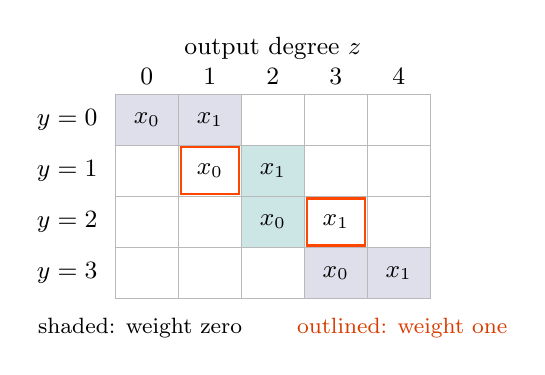
\begin{tikzpicture}[x=.8cm,y=.65cm,font=\small]
 \node at (2.5,4.9) {output degree \(z\)};
 \foreach \z in {0,...,4}{\node at (\z+.5,4.35) {\(\z\)};}
 \foreach \y in {0,...,3}{\node[anchor=east] at (-.13,3.5-\y) {\(y=\y\)};}
 \fill[MidnightBlue!14] (0,3) rectangle (2,4);
 \fill[teal!20] (2,1) rectangle (3,3);
 \fill[MidnightBlue!14] (3,0) rectangle (5,1);
 \draw[step=1,gray!55,thin] (0,0) grid (5,4);
 \foreach \y in {0,...,3}{\foreach \i in {0,1}{
   \node at (\y+\i+.5,3.5-\y) {\(x_{\i}\)};
 }}
 \draw[thick,OrangeRed] (1.04,2.04) rectangle (1.96,2.96);
 \draw[thick,OrangeRed] (3.04,1.04) rectangle (3.96,1.96);
 \node[below,align=center,font=\footnotesize] at (2.5,-.18) {shaded: weight zero \qquad \textcolor{OrangeRed!85!black}{outlined: weight one}};
\end{tikzpicture}
\caption{The three-sector degeneration at \(a=2,h=1\). The middle sector exploits the transposed convolution instead of leaving an unused gap between two outer sectors.}
\end{figure}

Applying the entropy inequality with uniform weights \(1/3\) gives
\[
 \phi_\pi(P_{a,B})\geq3^{p_X^{(\pi)}}
 \phi_\pi(P_{a,h})^{2/3}\phi_\pi(P_{a,h}^{(23)})^{1/3}.
\]
The permutation \((23)\) simply reorders the factors in the six-fold product. After normalization, the result is \eqref{eq:mm-nine-fourths-recurrence}.

\subsection{The diagonal growth and the origin of four thirds}

Define \(D_a=P(a,a)\) and \(\Delta_{a,j}=P(a,j+1)-P(a,j)\). Concavity makes \(\Delta_{a,j}\) nonincreasing in \(j\). Shifted tripling at \(h=a\) gives
\[
 2D_a\leq P(a,4a-1)-D_a
   =\sum_{j=a}^{4a-2}\Delta_{a,j}
   \leq(3a-1)\Delta_{a,a}.
\]
Let \(H_a=2D_a/(3a-1)\). Then \(\Delta_{a,a}\geq H_a\). By symmetry and concavity,
\[
 D_a-D_{a-1}=\Delta_{a-1,a-1}+\Delta_{a,a-1}
 \geq H_{a-1}+H_a.
\]
Substituting \(D_a=(3a-1)H_a/2\) and rearranging gives
\[
 H_a\geq\left(1+\frac{1}{3(a-1)}\right)H_{a-1},
 \qquad H_1=1.
\]
Since \((1+1/(3j))^3\geq1+1/j\), the product telescopes after cubing:
\[
 H_a^3\geq\prod_{j=1}^{a-1}(1+1/j)=a.
\]
Consequently \(D_a\geq aH_a\geq a^{4/3}\).

\begin{theorem}[The upper-bound squeeze]
\label{thm:mm-nine-fourths-upper}
Over every algebraically closed field, \(\omega\leq9/4\).
\end{theorem}
\begin{proof}
The diagonal estimate and interpolation give
\[
 a^{4/3}\leq P(a,a)\leq(2a-1)^{1/t}.
\]
Letting \(a\to\infty\) forces \(1/t\geq4/3\). Thus \(3t\leq9/4\) for every character, and asymptotic spectrum duality (Theorem~\ref{thm:mm-nine-fourths-strassen-duality}) yields the claimed bound.
\end{proof}

\begin{moral}
The \(9/4\) is not an optimization artifact: the three directional exponents are constrained by a convolution profile with forced diagonal growth \(a^{4/3}\). The quotient \(3/(4/3)=9/4\) is the resulting bound.
\end{moral}

\section{Elementary perspectives and arbitrary fields}

Sch\"onhage's asymptotic sum inequality gives another route from tensor degenerations to algorithms. If
\[
 \underline R\left(\bigoplus_i\langle n_i,m_i,p_i\rangle\right)\leq r,
 \quad\text{then}\quad \sum_i(n_i m_i p_i)^{\omega/3}\leq r.
\]
Pass gives a constructive proof of the \(9/4\) bound using composable polynomial packings. Do\u{g}an, Lysikov, Sakabe and Walter instead use a fractional symmetrized tensor value, which replaces spectral points while retaining the essential partially-direct-sum inequality.\footnote{R. Pass, \emph{Matrix Multiplication from Polynomial Packings: A Constructive and Elementary Proof of \(\omega\leq9/4\)}, \href{https://arxiv.org/abs/2610.28627}{arXiv:2610.28627}; M. L. Do\u{g}an, V. Lysikov, K. Sakabe and M. Walter, \emph{Tensor value and the \(9/4\) bound for matrix multiplication}, \href{https://arxiv.org/abs/2611.09716}{arXiv:2611.09716}.}

The Fourier argument above works over \(\overline{\FF}\), which has arbitrarily many interpolation points and roots of unity of order prime to its characteristic. For any \(\delta>0\), choose a fixed side \(s\) and a rank decomposition over \(\overline{\FF}\) with \(r<s^{9/4+\delta}\) terms. Its finitely many coefficients lie in a finite extension \(K/\FF\). Simulating arithmetic in \(K\) in a fixed \(\FF\)-basis costs a constant, independent of matrix size. Recursive block multiplication with this identity proves \(\omega_\FF\leq9/4+\delta\), and \(\delta\to0\) gives the all-fields bound.

There are also polynomial separation proofs avoiding the Fourier step.\footnote{H. L\"u, \emph{Polynomial Separation of a Shared Tensor Leg and Matrix Multiplication in Arbitrary Characteristic}, \href{https://arxiv.org/abs/2610.18914}{arXiv:2610.18914}; A. Amanov, M. van den Berg and J. Zuiddam, \emph{Multiplying matrices via polynomials: exposition and barriers}, \href{https://arxiv.org/abs/2610.30054}{arXiv:2610.30054}. The latter paper also proves a barrier for its particular collection of degeneration ingredients, not an unconditional lower bound for all algorithms.}

\section{The dual side: tensor networks and list distinctness}

The November 24, 2026 manuscript reduces the matching lower bound to a contradiction about the size of tensor networks representing a particular Boolean function.

\subsection{Why ordinary flattenings do not suffice}

A flattening \(T_{(1)}:U^*\to V\otimes W\) gives \(R(T)\geq\underline R(T)\geq\rank(T_{(1)})\). The matrix multiplication tensor has flattening rank exactly \(n^2\): its slices indexed by the first matrix entry have disjoint nonzero supports. A lower bound of order \(n^2\), even with a fixed constant-factor improvement, cannot distinguish an asymptotic exponent of \(2\) from one of \(9/4\).

\subsection{The tensor of list distinctness}

Fix a finite field \(k\). A bit tensor of arity \(u\) is a function \(\{0,1\}^u\to k\). A network contracts such tables by summing over internal wire assignments; named exterior wires remain as independent arguments. A trivalent network has arity at most three at every vertex. Its size counts vertices and exterior bits; its volume counts vertices and wires, quantities comparable up to an absolute constant.

For \(w\geq1\), let \(D_w\) be the zero-one tensor testing whether a list of \(2^w\) words of \(2w\) bits each has no repeated word. There are
\[
 n_w=2w\,2^w
\]
exterior bits. The power \(D_w^{\otimes t}\) tests \(t\) independent lists at once. Crucially, a network computing this tensor is permitted to connect vertices across the lists.

An initial trivalent network for \(D_w\) has size \(O(n_ww^2)\). A sorting network on \(2^w\) records requires \(O(2^w w^2)\) comparisons, each implemented with \(O(w)\) Boolean gates. After sorting, compare adjacent words. Encode gates as truth tables, fan-out as equality constraints, and pin the final output to \(1\). For accepted exterior bits there is exactly one consistent internal assignment, so the contraction equals \(1\) over any field.

\subsection{Two geometric estimates from the lower-bound manuscript}

The geometric part of the argument supplies the following two results. We use them as cited theorems: their proofs require the separate machinery of sphere tensors, prices, arity concentration and the list-distinctness obstruction developed in the manuscript. The reduction below is explicit and does not rely on a hypothetical network invariant.\footnote{OpenAI, \emph{The matrix multiplication exponent is nine fourths}, November 24, 2026, Section 2 and the later sections proving the compression and list-distinctness estimates; \href{https://github.com/openai/math/blob/main/preprints/The-matrix-multiplication-exponent-is-nine-fourths-November-24-2026/build/obstruction.tex}{statements and reduction}.}

\begin{theorem}[Tensor-power compression under a smaller exponent]
\label{thm:mm-nine-fourths-compression}
Assume \(\omega_k<9/4\). For any \(\eta>0\) there is \(\gamma>0\) such that for sufficiently large \(n\), writing \(h=\lceil\log_2 n\rceil\), a trivalent network of size \(m\leq n^{1.05}\) with \(e\geq n\) exterior bits representing \(V\) admits a network for some power \(V^{\otimes d}\) of size at most
\[
 d(mh^{-\gamma}+eh^\eta).
\]
The new network has \(de\) distinct exterior bits and \(d\leq n^{o(1)}\) uniformly for fixed \(k,\eta\).
\end{theorem}

\begin{theorem}[List-distinctness volume bound]
\label{thm:mm-nine-fourths-distinctness}
There exists \(\sigma>0\), depending on \(k\), such that for sufficiently large \(w\) and all \(1\leq t\leq2^w\),
\[
 \operatorname{vol}_k(D_w^{\otimes t})>t n_w w^\sigma.
\]
Here \(\operatorname{vol}_k\) is the minimum trivalent network volume.
\end{theorem}

The first estimate permits a logarithmic saving in size per copy while charging a smaller logarithmic power per exterior bit. The second says that this saving cannot push list-distinctness networks below a certain cost per bit, even if many copies are computed jointly. The uniformity in \(t\) is indispensable.

\subsection{A contradiction through amortized size}

\begin{proposition}
\label{prop:mm-nine-fourths-finite-lower}
The two preceding estimates imply \(\omega_k\geq9/4\) over every finite field.
\end{proposition}
\begin{proof}
Assume \(\omega_k<9/4\), choose \(0<\eta<\sigma\), and take the corresponding \(\gamma\). Fix an integer \(J>2/\gamma\). Put \(n=n_w\) and keep \(h=\lceil\log_2 n\rceil\) fixed.

After \(j\) compression rounds, denote the number of lists by \(t_j\), the network size by \(m_j\), and its amortized size by \(x_j=m_j/(t_j n)\). Initially \(t_0=1\) and \(x_0=O(w^2)\). The compression theorem gives
\[
 t_{j+1}=d_jt_j,\qquad
 x_{j+1}\leq h^{-\gamma}x_j+h^\eta.
\]
For every fixed \(j\leq J\), the uniform bound \(d_j\leq n^{o(1)}\) implies \(t_j=n^{o(1)}\). The recurrence gives \(x_j=O(w^2+h^\eta)\), so \(m_j=t_jnx_j\leq n^{1.05}\) for large \(w\). There are at least \(n\) exterior bits at every step; hence the hypotheses remain valid.

Unrolling the recurrence yields
\[
 x_J\leq h^{-J\gamma}x_0+
 h^\eta\sum_{i=0}^{J-1}h^{-i\gamma}=O(w^\eta),
\]
since \(h=w+O(\log w)\) and \(J\gamma>2\). Moreover \(t_J=n^{o(1)}\leq2^w\). The constructed network has volume \(O(t_J n_w w^\eta)\), contrary to the lower bound \(t_J n_w w^\sigma\) as \(w\to\infty\).
\end{proof}

\begin{figure}[htbp]
\centering
\begin{tikzpicture}[>=Stealth,font=\small]
 \draw[->,thick] (0,0)--(7.8,0) node[right] {round};
 \draw[->,thick] (0,0)--(0,3.4) node[above] {size per bit};
 \draw[thick,dashed,OrangeRed] (.2,1.35)--(7.3,1.35);
 
 \draw[very thick,MidnightBlue,->] (.5,3)--(2,2.35)--(3.5,1.7)--(5.1,1)--(6.8,.6);
 \foreach \x/\y in {.5/3,2/2.35,3.5/1.7,5.1/1,6.8/.6}{\fill[MidnightBlue] (\x,\y) circle(2pt);}
 
 
 \draw[dotted,gray] (6.8,0)--(6.8,.6);
 \node[below] at (6.8,0) {\(J\)};
 \node[below] at (.5,0) {\(0\)};
 \draw[very thick,MidnightBlue] (.2,-.82)--(.85,-.82);
 \node[anchor=west,font=\footnotesize] at (1,-.82) {Size per bit: \(O(w^2)\) to \(O(w^\eta)\)};
 \draw[thick,dashed,OrangeRed] (.2,-1.28)--(.85,-1.28);
 \node[anchor=west,font=\footnotesize] at (1,-1.28) {\(\Omega(w^\sigma)\) obstruction};
\end{tikzpicture}
\caption{The amortized network-size recurrence. The obstruction is uniform over the allowed number of lists, so replication cannot evade it. Vertical scale is schematic.}
\end{figure}

\subsection{From arbitrary formal circuits to finite fields}

Consider a formal arithmetic circuit with \(q\) nonscalar multiplication or division gates, computing the matrix product as a rational-function identity. Over the algebraic closure choose constant matrices \(A,B\) avoiding the finitely many denominator zeros. Substitute \(A+uX,B+vY\) with \(u^2=v^2=0\). An intermediate expression has expansion
\[
 f=f_{00}+uf_{10}+vf_{01}+uvf_{11}.
\]
At a product gate \(f=ab\),
\[
 f_{11}=a_{00}b_{11}+a_{11}b_{00}+a_{10}b_{01}+a_{01}b_{10}.
\]
At a quotient gate use \(bf=a\), so
\[
 f_{11}=b_{00}^{-1}(a_{11}-b_{11}f_{00}-b_{10}f_{01}-b_{01}f_{10}).
\]
Only two new products of linear forms are needed at either type of gate. The mixed output is \(XY\); thus its tensor rank is at most \(2q\).

An exponent below \(9/4\) over any field \(\FF\) would therefore furnish a fixed side \(s\) and a rank decomposition with \(r<s^{9/4}\) terms over \(\overline{\FF}\). Form the ring generated over \(\ZZ\) by the finitely many decomposition coefficients and reduce modulo a maximal ideal. All tensor identities have integer coefficients and survive this reduction.

The residue field is finite. A field finitely generated as a ring over \(\ZZ\) cannot have characteristic zero: Zariski's lemma would make it a number field, whose finitely many ring generators lie in a ring of algebraic integers with only finitely many rational primes inverted, contradicting the presence of every rational inverse. In positive characteristic the same lemma over the prime field gives a finite extension. The reduction therefore gives a length-\(r\) decomposition over a finite field \(k\). Recursive block multiplication implies \(\omega_k\leq\log_s r<9/4\), contradicting Proposition~\ref{prop:mm-nine-fourths-finite-lower}.

\subsection{Consequences of the claimed matching bound}

If the lower-bound manuscript's estimates hold, combining them with the upper bound gives \(\omega_\FF=9/4\). Every fixed-size rank decomposition must have at least \(n^{9/4}\) terms, because a shorter one would yield a smaller exponent by recursion. Bilinearization then forces at least \(\lceil n^{9/4}/2\rceil\) nonscalar multiplication or division gates. Applying the rank bound to all tensor powers and using the upper bound also gives
\[
 \widetilde R_\FF(\langle n,n,n\rangle)=n^{9/4}.
\]
These are formal algebraic complexity statements, not predictions about finite-size runtime. The lower-bound deduction above isolates the two deep geometric estimates on which the November claim rests.

\section{Open structural questions}

The proposed matching exponent raises several further structural questions:
\begin{enumerate}
  \item \textbf{Attainability of the infimum.} Does there exist a constant \(C\) (or polylogarithmic factor) such that \(R(\langle n, n, n \rangle) \le C n^{9/4} \operatorname{polylog}(n)\), or is the extra \(n^\delta\) overhead intrinsic to the asymptotic degeneration?
  \item \textbf{Rectangular matrix multiplication \(\omega(1, \kappa, 1)\).} Let \(\omega(\kappa)\) denote the exponent of multiplying an \(n \times n^\kappa\) matrix by an \(n^\kappa \times n\) matrix. How does the shared-leg separation framework reshape the curve \(\kappa \mapsto \omega(\kappa)\), and what becomes of the dual exponent \(\alpha = \sup\{\kappa : \omega(\kappa) = 2\}\)?
  \item \textbf{Scope of tensor-network incompressibility.} If the tensor-network obstruction extends to other complexity measures, what other multilinear families (such as iterated matrix multiplication, determinant, or permanent) fall within reach of the same geometric barrier?
\end{enumerate}
